\subsubsection{スイッチ}\label{switch}
\begin{table}[H]
	\begin{tabular}{|p{\colF}|p{\colG}|}	\hline
	名称 & スイッチ(すいっち)\\ \hline
	接続箇所 & デジタルコネクタ (3pin)\\ \hline
	機能概要 & ONとOFFを切りかえる\\ \hline
  \end{tabular}
\end{table}

\begin{table}[H]
	\begin{tabular}{|p{\colF}|p{\colG}|}	\hline
	サンプルコードの場所 & ome/05/digin.hsp\\ \hline
	raspiへの入力 & 右にスライドさせると1、左にスライドさせると0を入力する\\ \hline
	raspiへの入力方法 & val = gpioin(GPIO番号)\\ \hline
	raspiからの出力 & なし\\ \hline
	raspiからの出力方法 & なし\\ \hline
  \end{tabular}
\end{table}

\begin{table}[H]
	\begin{tabular}{|p{\colF}|p{\colG}|} \hline
	使い道 & 照明のスイッチ\\ \hline
	注意事項 & なし\\ \hline
	補足 & ボタンと違い、人の手を使わなくとも値を保持しておくことができます。\\ \hline
  \end{tabular}
\end{table}

\begin{figure}[H]
	\begin{tabular}{|p{\colH}|p{\colI}|p{\colH}|p{\colI}|} \hline
	外観 & 
	\begin{minipage}[t]{\linewidth}
    \smallskip
      \centering
      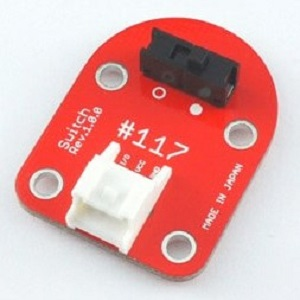
\includegraphics[width=\linewidth]{images/chap05/text05-img019.jpg}
      \caption{スイッチ}
      \smallskip
    \end{minipage} &
    回路記号 & 
    \begin{minipage}[t]{\linewidth}
    \smallskip
      \centering
      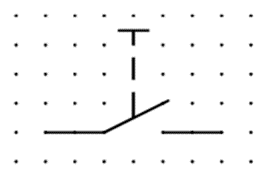
\includegraphics[width=\linewidth]{images/chap05/text05-img047.png}
      \caption{スイッチの回路図}
      \smallskip
    \end{minipage}\\ \hline
  \end{tabular}
\end{figure}